\documentclass[12pt]{article}
\usepackage[utf8x]{inputenc}
\usepackage{float}
\usepackage[francais]{babel}
\usepackage{graphicx}
\usepackage{amsmath}
\usepackage{hyperref}
\usepackage[
        a4paper,
        left=2.5cm,
        right=2.5cm,
        top=2cm,
        bottom=2.5cm,
]{geometry}

%% TITRE
\title{Randomized Kinodynamic Planning\\
\textsc{\small École Normale Supérieure Paris-Saclay}}
\author{Olivier Lévêque \& Aboubacar Tuo}
\date{\today}

%% CONTENU
\begin{document}
\maketitle

\begin{abstract}
Ce rapport a pour étude l'article \textbf{Randomized Kinodynamic Planning} écrit par Steven M. LaValle et James J. Kuffner, Jr. en 1999. Un résumé de l'article et des simulations de l'algorithme RRT vous sont proposés.
\begin{center}
\url{http://msl.cs.uiuc.edu/~lavalle/papers/LavKuf01b.pdf}
\end{center}
\end{abstract}

\section{Introduction}

\paragraph{}
Cet article\footnote{\url{http://msl.cs.uiuc.edu/~lavalle/papers/LavKuf01b.pdf}} présente la première approche pour la planification probabiliste de trajectoires, connue aussi sous le nom de \og kinodynamic planning \fg{}. Ce terme, introduit par B. Donald, P. Xavier, J. Canny et J. Rief en 1993 dans une de leurs publications \textbf{Kinodynamic motion planning} dans le \textit{Journal of the ACM}, décrit une famille de problèmes fondamentaux cherchant à construire une trajectoire en boucle ouverte satisfaisant à la fois les contraintes imposées par des obstacles environnants mais aussi des contraintes différentielles locales imposées par la dynamique du système étudié.

\paragraph{}
Il est intéressant de noter que la planification de trajectoire peut être utilisée dans tous les domaines faisant appel à des modèles théoriques pour le contrôle de systèmes dynamiques. Ces domaines sont très variés, allant des préhenseurs en robotique aux modèles d'économétrie. De nombreux secteurs industriels font appel à la planification de trajectoire comme par exemple l'industrie cinématographique pour des effets visuels avancés (mouvements d'objets et de personnes obéissant aux lois physiques).

\paragraph{}
L'approche classique de la planification repose sur le découpage du problème général en trois parties.
\begin{enumerate}
\item	Résoudre le problème de planification de base ;
\item	Trouver une trajectoire et une commande satisfaisant la dynamique du système ;
\item	Suivre cette trajectoire.
\end{enumerate}

\paragraph{}
La majorité des algorithmes permettant de résoudre le problème de planification repose uniquement sur la cinématique du système et ignore complètement sa dynamique. C'est pourquoi le problème kinodynamique, qui prend compte de cette dynamique, est considéré comme une généralisation du problème de la planification holonome et non-holonome dans l'espace des variables d'état.


\section{Formulation du problème}

\paragraph{}
Le problème de planification kinodynamique est formulé comme un problème de planification dans l'espace des variables d'état avec des contraintes différentielles d'ordre 1. Posons $\mathcal{C}$ l'espace des configurations pour un système rigide ou articulé pouvant se déplacer en 2D ou 3D, tel que chaque configuration $q \in \mathcal{C}$ représente une transformation appliquée au modèle géométrique associé au système. Posons aussi $\mathcal{X}$ l'espace d'état, tel que $x \in \mathcal{X}$ s'écrive $x=(q,\dot{q})$.

\paragraph{}
Sous des conditions appropriées\footnote{Conditions du théorème des fonctions implicites}, les contraintes différentielles peut-être exprimées sous la forme
\begin{equation}
\label{eqdiff}
\dot{x}=f(x,u) \text{ avec } u \in \mathcal{U}
\end{equation}
où $\mathcal{U}$ représente l'ensemble des commandes admissibles.

\paragraph{}
Si nous considérons un environnement contenant des obstacles statiques. Il existe des différences notables entre trouver un chemin sans collision dans $\mathcal{C}$ ou dans $\mathcal{X}$. Dans $\mathcal{C}$, nous pouvons caractériser l'ensemble des configurations $\mathcal{C}_{obst}$ où le robot est en collision. La planification de trajectoire implique de trouver un chemin continu dans l'ensemble $\mathcal{C}_{free}$ tel que $\mathcal{C}_{free}=\mathcal{C}\setminus\mathcal{C}_{obst}$. Dans $\mathcal{X}$, nous pouvons définir $\mathcal{X}_{obst}$ tel que $x \in \mathcal{X}_{obst}$ si et seulement si $q_{obst} \in \mathcal{C}$ pour $x=(q, \dot{q})$, cependant en considérant la dynamique du système, une autre région interdite existe : \textit{la région des collisions inévitables} que nous noterons $\mathcal{X}_{ric}$. Cette région correspond aux états où il n'existe aucune commande pour éviter la collision. Nous pouvons noter que $\mathcal{X}_{obst} \subseteq \mathcal{X}_{ric}$.\\
L'ensemble $\mathcal{X}_{ric}$ traduit bien la difficulté du problème de planification kinodynamique car si une trajectoire cinématique sans collision existe à un problème de planification, une trajectoire kinodynamique n'existe quant à elle pas forcément. Comme dans l'article, nous définirons $\mathcal{X}_{free} = \mathcal{X}\setminus\mathcal{X}_{obst}$ bien que la définition $\mathcal{X}_{free} = \mathcal{X}\setminus\mathcal{X}_{ric}$ est aussi une alternative possible.

\paragraph{}
Avec cette définition de  $\mathcal{X}_{free}$, résoudre le problème de planification kinodynamique revient à  trouver une trajectoire d'un état initial, $x_{init} \in \mathcal{X}_{free}$, à un état final, $x_{goal} \in \mathcal{X}_{free}$ telle que cette trajectoire soit un chemin continu paramétré en temps, $\tau : [0,T] \longrightarrow \mathcal{X}_{free}$.\\
L'état final peut aussi être considéré comme une région de l'espace d'état, tel que $\mathcal{X}_{goal} \subset \mathcal{X}_{free}$.

\paragraph{}
La trajectoire, $x(t)$ pour $t \in [0,T]$, est déterminée en intégrant l'équation \eqref{eqdiff}. Il peut être approprié de sélectionner la trajectoire qui optimise un certain critère tel que la distance nécessaire pour atteindre $x_{goal}$.

\paragraph{}
Une approximation numérique de l'équation \eqref{eqdiff} pour calculer l'état suivant $x(t+\delta t)$ à partir de l'état actuel $x(t)$ et de la commande $u(t')$ avec $t' \in [t, t+\delta t]$ est, par exemple, de choisir une commande $u$ constante sur l'intervalle d'intégration $[t, t+\delta t]$ et d'utiliser la méthode d'intégration de Runge-Kutta d'ordre 4.

$$
x(t+\delta t) \approx x(t)+\frac{\delta t}{6}(f(x(t),u)+2x'+2x''+x''') \text{ avec } \left\{
\begin{matrix}
x' &= f(x(t)+\frac{\delta t}{2}x,u)\\
x'' &= f(x(t)+\frac{\delta t}{2}x',u)\\
x''' &= f(x(t)+\frac{\delta t}{2}x'',u)
\end{matrix}
\right.
$$


\section{Rapidly-Exploring Random Trees (RRT)}

\paragraph{}
Les auteurs de l'article proposent pour résoudre le problème de plannification kinodynamique un algorithme baptisé \og Rapidly-Exploring Random Trees \fg{} (RRT). Il s'agit d'une méthode simple permettant d'explorer de manière rapide, aléatoire et uniforme l'espace d'état.

\begin{figure}[H]
\centering
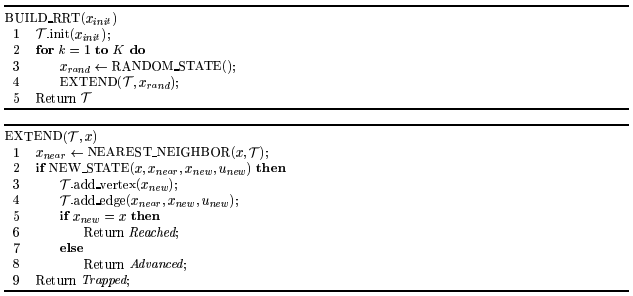
\includegraphics[scale=0.65]{img/RRTalgo.png}
\caption{Structure de l'algorithme RRT}
\label{RRTalgo}
\end{figure}

\paragraph{}
Pour cette exploration, l'algorithme RRT construit un arbre de la manière suivante. Il commence par définir l'état initial $x_{init}$ comme un sommet de l'arbre puis répétitivement tire aléatoirement un échantillon $x$ dans l'espace d'état, cherche selon une métrique $\rho$ le sommet voisin le plus proche, $x^{near}_k$ (fonction EXTEND -- figure \ref{EXTEND}) et trouve un contrôle $u_k \in \mathcal{U}$ permettant, à partir de $x^{near}_k$, de se rapprocher de $x$ (fonction NEW\_STATE). Alors $x^{new}_{k+1} = f(x^{near}_k,u_k)$ est ajouté à l'arbre s'il respecte bien les contraintes globales\footnote{L'état $x^{new}_{k+1}$ doit appartenir à $\mathcal{X}_{free}$}. La structure de l'algorithme RRT est rappelée figure \ref{RRTalgo}.

\begin{figure}[H]
\centering
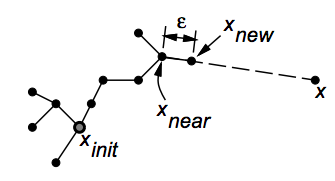
\includegraphics[scale=0.7]{img/EXTEND.png}
\caption{L'opération EXTEND}
\label{EXTEND}
\end{figure}

\paragraph{}
La commande $u_k \in \mathcal{U}$ est appliquée durant un temps $\Delta t$ qui peut-être choisi fixe ou aléatoire à chaque itération dans un intervalle $]0,\Delta t_{max}]$. En général, $\Delta t$ doit être bien plus grand que le temps d'intégration $\delta t$ nécessaire pour calculer \eqref{eqdiff}. La commande $u_k$ peut-être choisi aléatoirement ou en essayant toutes les possibilités et en gardant celle qui rapproche le plus possible le nouveau sommet $x^{new}_{k+1}$ de l'échantillon $x$. Si $\mathcal{U}$ est infini, l'ensemble peut être discrétisé. L'échantillon $x$ est considéré comme atteint si $||x^{new}_{k+1}-x||<\epsilon$ avec $\epsilon>0$.

\paragraph{}
Pour construire une trajectoire à partir de l'exploration précédente, nous devons construire deux arbres RRT l'un partant de l'état initial, $x_{init}$ et l'autre de l'état final, $x_{goal}$. Cette algorithme, baptisé \og RRT bidirectionnel \fg{}, cherche les sommets communs aux deux arbres. Deux sommets, $x$ et $x'$, sont considérés en commun si $\rho(x,x')<\epsilon$ avec $\epsilon>0$. L'algorithme peut s'arrêter au premier couple de sommets communs trouvé ou peut continuer pour choisir la meilleure trajectoire parmis la collection de sommets communs trouvés. La structure de l'algorithme RRT bidirectionnel est rappelée figure \ref{RRTbi}.

\begin{figure}[H]
\centering
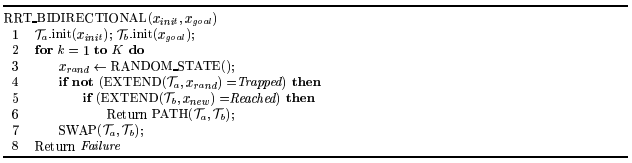
\includegraphics[scale=0.65]{img/RRTbi.png}
\caption{Structure de l'algorithme RRT bidirectionnel}
\label{RRTbi}
\end{figure}

\section{Implémentations \& Simulations}

\paragraph{}
Plusieurs simulations de planification kinodynamique ont été menées par nos soins sous MATLAB, et vous sont présentées dans cette section. La figure \ref{RRTStar} illustre l'exploration d'un espace d'état à l'aide de l'algorithme RRT détaillé précédemment et la figure \ref{RRTBi} illustre le fonctionnement de l'algorithme RRT bidirectonnel pour la recherche d'une trajectoire kinodynamique entre un état initial $x_{init} \in \mathcal{X}_{free}$ et un état final $x_{goal} \in \mathcal{X}_{free}$.

\paragraph{Dynamique du modèle} Le système rigide considéré ici est une voiture se déplaçant en 2D, ne pouvant qu'avancer (pas de marche arrière) et tourner. Sa dynamique est fournie par les équations suivantes.
\begin{align*}
x &= \begin{pmatrix}
p_1\\ p_2\\ \theta
\end{pmatrix} \in \mathcal{X}\\
\dot{x} = f(x(t),u(t)) &= \begin{pmatrix}
\dot{p_1}\\ \dot{p_2}\\ \dot{\theta}
\end{pmatrix} = \begin{pmatrix}
u_1 \cos(u_2)\\ u_1 \sin(u_2)\\ u_2
\end{pmatrix} \in \mathcal{C}
\end{align*}

avec

\begin{align*}
\mathcal{X}&=[0,100]\times[0,100]\times[-\pi,\pi[
\end{align*}

\paragraph{Métrique} Pour pouvoir calculer une distance entre différents états, nous nous munissons de la métrique suivante correspondant à la norme euclidienne.
\begin{align*}
\rho(x_1,x_2) &= \sqrt{\alpha(p_{1,1}-p_{1,2})^2+\beta(p_{2,1}-p_{2,2})^2+\gamma(\theta_1-\theta_2)^2}
\end{align*}

où $\alpha$, $\beta$ et $\gamma$ sont respectivement les poids des composantes $p_{1,i}$ (position horizontal), $p_{2,i}$ (position verticale) et $\theta_i$ (position angulaire) des états $x_i$. Nous avons choisi ici $\alpha = \beta = 1$ et $\gamma = 0$ pour calculer la distance séparant deux positions spatiales de la voiture.

\paragraph{Commande appliquée} Pour calculer la commande $u=(u_1,u_2) \in \mathcal{U}$ connaissant le sommet voisin $x^{near}$ et l'échantillon $x$ que nous cherchons à atteindre, nous calculons la commande $u$ comme recommandé dans la section $5.5$ du livre de Steven M. LaValle\footnote{\url{http://planning.cs.uiuc.edu/}}.

\begin{align*}
u_1 &= \frac{\rho(x^{near},x)}{M} \text{ avec } M=100\\
u_2 &= \arctan\left(\frac{p_{2,x}-p_{2,x_k^{near}}}{p_{1,x}-p_{1,x_k^{near}}}\right)
\end{align*}

$M$ est ici un facteur de normalisation choisi pour que $u_1$ appartient à l'intervalle $[0,1]$. Nous constatons qu'avec cette approche, au fur et à mesure que l'échantillon $x$ tiré est proche d'un des sommets de l'arbre, $\rho(x^{near},x)$ devient petit. Ainsi $u_1$ impose de petits déplacements à la voiture permettant une meilleur exploration de l'espace d'état $\mathcal{X}$.

\begin{figure}[H]
\centering
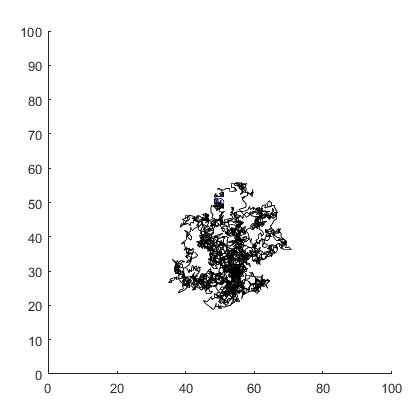
\includegraphics[width=0.45\textwidth]{../matlab/native.png}
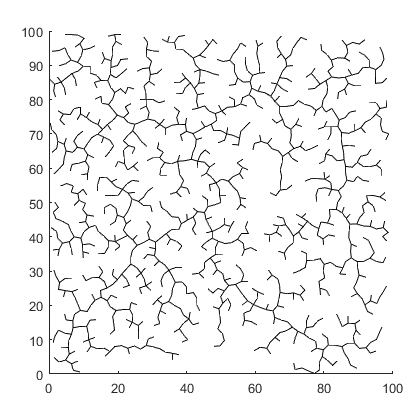
\includegraphics[width=0.45\textwidth]{../matlab/RRTexplore.png}
\caption{Comparaison entre un algorithme d'exploration naïf (à gauche) et l'algorithme d'exploration RRT (à droite) -- L'algorithme d'exploration naïf consiste à explorer l'espace d'état avec un pas fixe et une direction aléatoire recalculée à chaque itération. Nous constatons qu'avec le même nombre d'itérations (3000) et le même état initial (50,50), l'algorithme RRT explore plus rapidement et de manière uniforme l'espace d'état.}
\label{RRTStar}
\end{figure}


\begin{figure}[H]
\centering
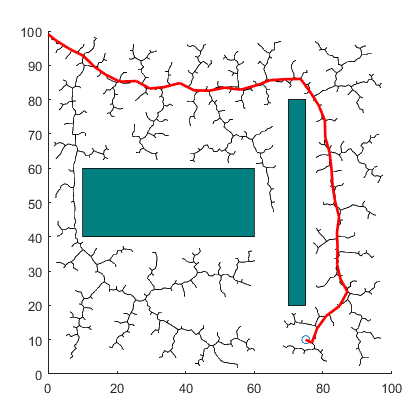
\includegraphics[width=0.45\textwidth]{../matlab/Traj_RRT.png}
\includegraphics[width=0.45\textwidth]{../matlab/Traj_RRTbi.png}
\caption{Comparaison entre une trajectoire kinodynamique déterminée à l'aide de l'algorithme RRT (à gauche) et RTT bidirectionnel (à droite) partant du même état initial (1,99) et arrivant au même état final (75,10) -- L'algorithme RTT bidirectionnel trouve une trajectoire plus rapidement et avec une exploration moins approfondie que l'algorithme RRT.}
\label{RRTBi}
\end{figure}

Lors de l'exploration figure \ref{RRTBi} (à gauche), nous associons à chaque sommet un coût correspondant à la distance parcourue sur l'arbre depuis le sommet initial. Pour calculer la trajectoire de coût minimal, nous définissons pour chaque sommet un \og parent \fg{} correspondant au sommet voisin de coût minimal. Nous pouvons ainsi construire la trajectoire optimale\footnote{Trajectoire de coût minimal} en partant de l'état final et en remontant de parent en parent jusqu'à l'état initial. 

\section{Conclusion}
Ce rapport, résumé de l'article \textbf{Randomized Kinodynamic Planning} écrit par Steven M. LaValle et James J. Kuffner, aura permis de rappeler l'intérêt et la formulation du problème de planification kinodynamique en décrivant l'algorithme \og Rapidly-Exploring Random Trees \fg{}  (RRT) permettant une exploration rapide, aléatoire et uniforme de l'espace d'état et l'algorithme RRT bidirectionnel permettant de trouver une trajectoire dans l'espace d'état issue de cette exploration.

\end{document}